\documentclass{article}
% Use the TikZ bounding box as the PDF page size (pdfLaTeX).
\usepackage{tikz}
\newsavebox{\plotbox}
\newcommand{\startplot}{\begin{lrbox}{\plotbox}\ignorespaces}
\newcommand{\finishplot}{\unskip\end{lrbox}%
  \pdfhorigin=2pt\pdfvorigin=2pt
  \pdfpagewidth=\dimexpr\wd\plotbox+4pt\relax
  \pdfpageheight=\dimexpr\ht\plotbox+\dp\plotbox+4pt\relax
  \shipout\box\plotbox}

\usetikzlibrary{arrows.meta}
\definecolor{ink}{HTML}{263B43}
\definecolor{sub}{HTML}{506269}
\definecolor{grid}{HTML}{DCE3E4}
\definecolor{axis}{HTML}{8A999D}
\definecolor{c0}{HTML}{475A78}
\definecolor{c1}{HTML}{5492B0}
\definecolor{c2}{HTML}{398678}
\definecolor{c3}{HTML}{AA7D37}
\definecolor{c4}{HTML}{AD4A34}
\begin{document}\startplot
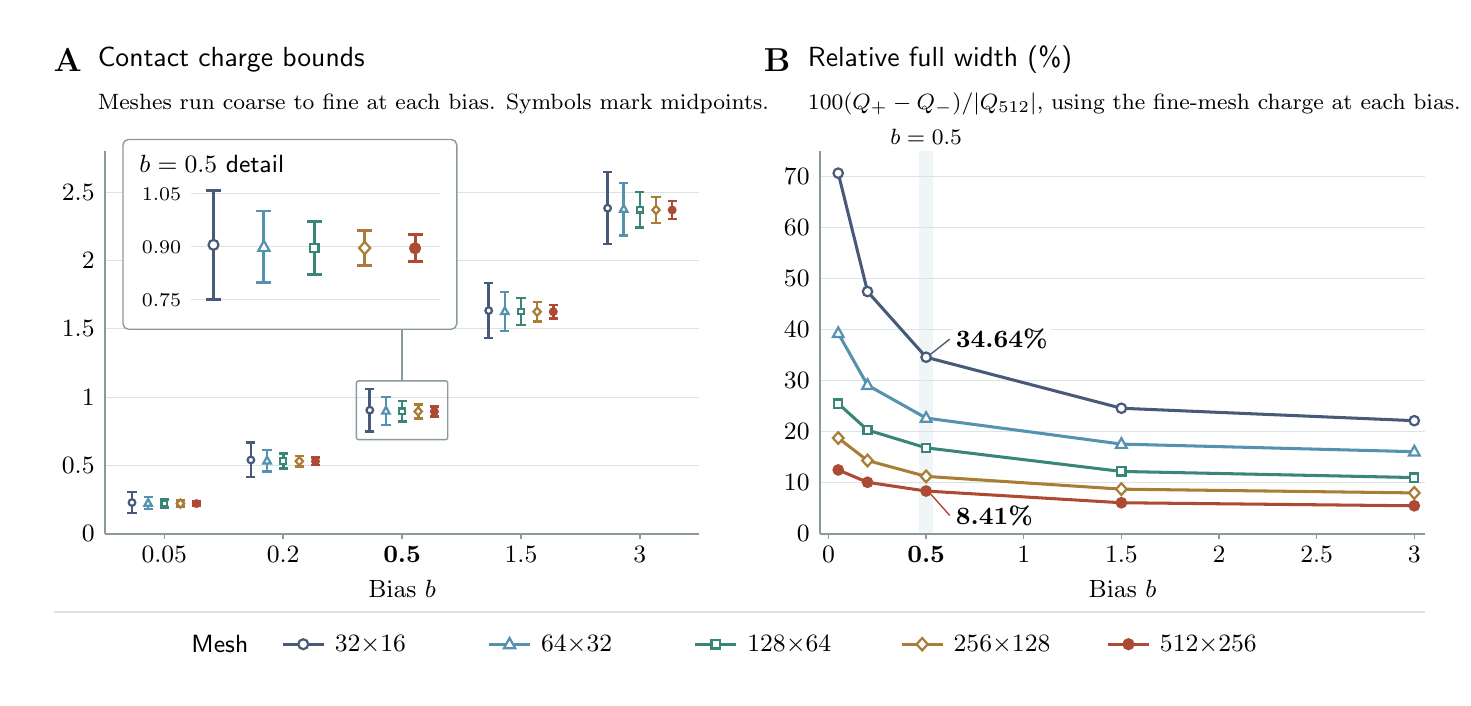
\begin{tikzpicture}[x=1cm,y=1cm,inner sep=0pt,outer sep=0pt,text=black]
\path[use as bounding box] (0,0) rectangle (17.97,8.26);
\node[anchor=west,font=\bfseries\large,text=black] at (0.3300,7.8500) {A};
\node[anchor=west,font=\sffamily\normalsize] at (0.8900,7.8500) {Contact charge bounds};
\node[anchor=west,font=\bfseries\large,text=black] at (9.3500,7.8500) {B};
\node[anchor=west,font=\sffamily\normalsize] at (9.9100,7.8500) {Relative full width (\%)};
\node[anchor=west,font=\footnotesize,text=black] at (0.8900,7.2900) {Meshes run coarse to fine at each bias. Symbols mark midpoints.};
\node[anchor=west,font=\footnotesize,text=black] at (9.9100,7.2900) {$100(Q_+-Q_-)/|Q_{512}|$, using the fine-mesh charge at each bias.};
\fill[c1!9] (11.3200,1.83) rectangle (11.5000,6.69);
\draw[axis,line width=.57pt] (0.9800,1.8300) -- (8.5300,1.8300);
\node[anchor=east,font=\small,text=black] at (0.8500,1.8300) {0};
\draw[grid,line width=.36pt] (0.9800,2.6979) -- (8.5300,2.6979);
\node[anchor=east,font=\small,text=black] at (0.8500,2.6979) {0.5};
\draw[grid,line width=.36pt] (0.9800,3.5657) -- (8.5300,3.5657);
\node[anchor=east,font=\small,text=black] at (0.8500,3.5657) {1};
\draw[grid,line width=.36pt] (0.9800,4.4336) -- (8.5300,4.4336);
\node[anchor=east,font=\small,text=black] at (0.8500,4.4336) {1.5};
\draw[grid,line width=.36pt] (0.9800,5.3014) -- (8.5300,5.3014);
\node[anchor=east,font=\small,text=black] at (0.8500,5.3014) {2};
\draw[grid,line width=.36pt] (0.9800,6.1693) -- (8.5300,6.1693);
\node[anchor=east,font=\small,text=black] at (0.8500,6.1693) {2.5};
\draw[axis,line width=.5pt] (0.9800,1.8300) -- (0.9800,6.6900);
\draw[axis,line width=.57pt] (10.0600,1.8300) -- (17.7500,1.8300);
\node[anchor=east,font=\small,text=black] at (9.9300,1.8300) {0};
\draw[grid,line width=.36pt] (10.0600,2.4780) -- (17.7500,2.4780);
\node[anchor=east,font=\small,text=black] at (9.9300,2.4780) {10};
\draw[grid,line width=.36pt] (10.0600,3.1260) -- (17.7500,3.1260);
\node[anchor=east,font=\small,text=black] at (9.9300,3.1260) {20};
\draw[grid,line width=.36pt] (10.0600,3.7740) -- (17.7500,3.7740);
\node[anchor=east,font=\small,text=black] at (9.9300,3.7740) {30};
\draw[grid,line width=.36pt] (10.0600,4.4220) -- (17.7500,4.4220);
\node[anchor=east,font=\small,text=black] at (9.9300,4.4220) {40};
\draw[grid,line width=.36pt] (10.0600,5.0700) -- (17.7500,5.0700);
\node[anchor=east,font=\small,text=black] at (9.9300,5.0700) {50};
\draw[grid,line width=.36pt] (10.0600,5.7180) -- (17.7500,5.7180);
\node[anchor=east,font=\small,text=black] at (9.9300,5.7180) {60};
\draw[grid,line width=.36pt] (10.0600,6.3660) -- (17.7500,6.3660);
\node[anchor=east,font=\small,text=black] at (9.9300,6.3660) {70};
\draw[axis,line width=.5pt] (10.0600,1.8300) -- (10.0600,6.6900);
\draw[axis,line width=.5pt] (1.7350,1.8300) -- (1.7350,1.7600);
\node[font=\small,text=black] at (1.7350,1.5700) {0.05};
\draw[axis,line width=.5pt] (3.2450,1.8300) -- (3.2450,1.7600);
\node[font=\small,text=black] at (3.2450,1.5700) {0.2};
\draw[axis,line width=.5pt] (4.7550,1.8300) -- (4.7550,1.7600);
\node[font=\small\bfseries,text=black] at (4.7550,1.5700) {0.5};
\draw[axis,line width=.5pt] (6.2650,1.8300) -- (6.2650,1.7600);
\node[font=\small,text=black] at (6.2650,1.5700) {1.5};
\draw[axis,line width=.5pt] (7.7750,1.8300) -- (7.7750,1.7600);
\node[font=\small,text=black] at (7.7750,1.5700) {3};
\draw[axis,line width=.5pt] (10.1700,1.8300) -- (10.1700,1.7600);
\node[font=\small,text=black] at (10.1700,1.5700) {0};
\draw[axis,line width=.5pt] (11.4100,1.8300) -- (11.4100,1.7600);
\node[font=\small\bfseries,text=black] at (11.4100,1.5700) {0.5};
\draw[axis,line width=.5pt] (12.6500,1.8300) -- (12.6500,1.7600);
\node[font=\small,text=black] at (12.6500,1.5700) {1};
\draw[axis,line width=.5pt] (13.8900,1.8300) -- (13.8900,1.7600);
\node[font=\small,text=black] at (13.8900,1.5700) {1.5};
\draw[axis,line width=.5pt] (15.1300,1.8300) -- (15.1300,1.7600);
\node[font=\small,text=black] at (15.1300,1.5700) {2};
\draw[axis,line width=.5pt] (16.3700,1.8300) -- (16.3700,1.7600);
\node[font=\small,text=black] at (16.3700,1.5700) {2.5};
\draw[axis,line width=.5pt] (17.6100,1.8300) -- (17.6100,1.7600);
\node[font=\small,text=black] at (17.6100,1.5700) {3};
\node[font=\small,text=black] at (4.7550,1.1300) {Bias $b$};
\node[font=\small,text=black] at (13.9050,1.1300) {Bias $b$};
\draw[c0,line width=.95pt] (1.3250,2.0932) -- (1.3250,2.3657);
\draw[c0,line width=.9pt] (1.2670,2.0932) -- (1.3830,2.0932);
\draw[c0,line width=.9pt] (1.2670,2.3657) -- (1.3830,2.3657);
\path[draw=c0,line width=.80pt,fill=white] (1.32500,2.22945) circle[radius=0.04200cm];
\draw[c0,line width=.95pt] (2.8350,2.5504) -- (2.8350,2.9887);
\draw[c0,line width=.9pt] (2.7770,2.5504) -- (2.8930,2.5504);
\draw[c0,line width=.9pt] (2.7770,2.9887) -- (2.8930,2.9887);
\path[draw=c0,line width=.80pt,fill=white] (2.83500,2.76954) circle[radius=0.04200cm];
\draw[c0,line width=.95pt] (4.3450,3.1327) -- (4.3450,3.6713);
\draw[c0,line width=.9pt] (4.2870,3.1327) -- (4.4030,3.1327);
\draw[c0,line width=.9pt] (4.2870,3.6713) -- (4.4030,3.6713);
\path[draw=c0,line width=.80pt,fill=white] (4.34500,3.40200) circle[radius=0.04200cm];
\draw[c0,line width=.95pt] (5.8550,4.3195) -- (5.8550,5.0144);
\draw[c0,line width=.9pt] (5.7970,4.3195) -- (5.9130,4.3195);
\draw[c0,line width=.9pt] (5.7970,5.0144) -- (5.9130,5.0144);
\path[draw=c0,line width=.80pt,fill=white] (5.85500,4.66692) circle[radius=0.04200cm];
\draw[c0,line width=.95pt] (7.3650,5.5111) -- (7.3650,6.4238);
\draw[c0,line width=.9pt] (7.3070,5.5111) -- (7.4230,5.5111);
\draw[c0,line width=.9pt] (7.3070,6.4238) -- (7.4230,6.4238);
\path[draw=c0,line width=.80pt,fill=white] (7.36500,5.96746) circle[radius=0.04200cm];
\draw[c0,line width=1.1pt,line join=round] (10.29400,6.41229) -- (10.66600,4.90873) -- (11.41000,4.07461) -- (13.89000,3.42675) -- (17.61000,3.26877);
\path[draw=c0,line width=.80pt,fill=white] (10.29400,6.41229) circle[radius=0.06000cm];
\path[draw=c0,line width=.80pt,fill=white] (10.66600,4.90873) circle[radius=0.06000cm];
\path[draw=c0,line width=.80pt,fill=white] (11.41000,4.07461) circle[radius=0.06000cm];
\path[draw=c0,line width=.80pt,fill=white] (13.89000,3.42675) circle[radius=0.06000cm];
\path[draw=c0,line width=.80pt,fill=white] (17.61000,3.26877) circle[radius=0.06000cm];
\draw[c1,line width=.95pt] (1.5300,2.1458) -- (1.5300,2.2973);
\draw[c1,line width=.9pt] (1.4720,2.1458) -- (1.5880,2.1458);
\draw[c1,line width=.9pt] (1.4720,2.2973) -- (1.5880,2.2973);
\path[draw=c1,line width=.80pt,fill=white] (1.53000,2.27402) -- (1.48254,2.18792) -- (1.57746,2.18792) -- cycle;
\draw[c1,line width=.95pt] (3.0400,2.6252) -- (3.0400,2.8943);
\draw[c1,line width=.9pt] (2.9820,2.6252) -- (3.0980,2.6252);
\draw[c1,line width=.9pt] (2.9820,2.8943) -- (3.0980,2.8943);
\path[draw=c1,line width=.80pt,fill=white] (3.04000,2.81227) -- (2.99254,2.72617) -- (3.08746,2.72617) -- cycle;
\draw[c1,line width=.95pt] (4.5500,3.2152) -- (4.5500,3.5685);
\draw[c1,line width=.9pt] (4.4920,3.2152) -- (4.6080,3.2152);
\draw[c1,line width=.9pt] (4.4920,3.5685) -- (4.6080,3.5685);
\path[draw=c1,line width=.80pt,fill=white] (4.55000,3.44435) -- (4.50254,3.35825) -- (4.59746,3.35825) -- cycle;
\draw[c1,line width=.95pt] (6.0600,4.4079) -- (6.0600,4.9048);
\draw[c1,line width=.9pt] (6.0020,4.4079) -- (6.1180,4.4079);
\draw[c1,line width=.9pt] (6.0020,4.9048) -- (6.1180,4.9048);
\path[draw=c1,line width=.80pt,fill=white] (6.06000,4.70887) -- (6.01254,4.62277) -- (6.10746,4.62277) -- cycle;
\draw[c1,line width=.95pt] (7.5700,5.6235) -- (7.5700,6.2863);
\draw[c1,line width=.9pt] (7.5120,5.6235) -- (7.6280,5.6235);
\draw[c1,line width=.9pt] (7.5120,6.2863) -- (7.6280,6.2863);
\path[draw=c1,line width=.80pt,fill=white] (7.57000,6.00742) -- (7.52254,5.92132) -- (7.61746,5.92132) -- cycle;
\draw[c1,line width=1.1pt,line join=round] (10.29400,4.37838) -- (10.66600,3.71983) -- (11.41000,3.30213) -- (13.89000,2.97161) -- (17.61000,2.87477);
\path[draw=c1,line width=.80pt,fill=white] (10.29400,4.45338) -- (10.22620,4.33038) -- (10.36180,4.33038) -- cycle;
\path[draw=c1,line width=.80pt,fill=white] (10.66600,3.79483) -- (10.59820,3.67183) -- (10.73380,3.67183) -- cycle;
\path[draw=c1,line width=.80pt,fill=white] (11.41000,3.37713) -- (11.34220,3.25413) -- (11.47780,3.25413) -- cycle;
\path[draw=c1,line width=.80pt,fill=white] (13.89000,3.04661) -- (13.82220,2.92361) -- (13.95780,2.92361) -- cycle;
\path[draw=c1,line width=.80pt,fill=white] (17.61000,2.94977) -- (17.54220,2.82677) -- (17.67780,2.82677) -- cycle;
\draw[c2,line width=.95pt] (1.7350,2.1686) -- (1.7350,2.2670);
\draw[c2,line width=.9pt] (1.6770,2.1686) -- (1.7930,2.1686);
\draw[c2,line width=.9pt] (1.6770,2.2670) -- (1.7930,2.2670);
\path[draw=c2,line width=.80pt,fill=white] (1.69888,2.18167) -- (1.77112,2.18167) -- (1.77112,2.25391) -- (1.69888,2.25391) -- cycle;
\draw[c2,line width=.95pt] (3.2450,2.6611) -- (3.2450,2.8490);
\draw[c2,line width=.9pt] (3.1870,2.6611) -- (3.3030,2.6611);
\draw[c2,line width=.9pt] (3.1870,2.8490) -- (3.3030,2.8490);
\path[draw=c2,line width=.80pt,fill=white] (3.20888,2.71889) -- (3.28112,2.71889) -- (3.28112,2.79113) -- (3.20888,2.79113) -- cycle;
\draw[c2,line width=.95pt] (4.7550,3.2556) -- (4.7550,3.5181);
\draw[c2,line width=.9pt] (4.6970,3.2556) -- (4.8130,3.2556);
\draw[c2,line width=.9pt] (4.6970,3.5181) -- (4.8130,3.5181);
\path[draw=c2,line width=.80pt,fill=white] (4.71888,3.35072) -- (4.79112,3.35072) -- (4.79112,3.42296) -- (4.71888,3.42296) -- cycle;
\draw[c2,line width=.95pt] (6.2650,4.4821) -- (6.2650,4.8277);
\draw[c2,line width=.9pt] (6.2070,4.4821) -- (6.3230,4.4821);
\draw[c2,line width=.9pt] (6.2070,4.8277) -- (6.3230,4.8277);
\path[draw=c2,line width=.80pt,fill=white] (6.22888,4.61879) -- (6.30112,4.61879) -- (6.30112,4.69103) -- (6.22888,4.69103) -- cycle;
\draw[c2,line width=.95pt] (7.7750,5.7214) -- (7.7750,6.1759);
\draw[c2,line width=.9pt] (7.7170,5.7214) -- (7.8330,5.7214);
\draw[c2,line width=.9pt] (7.7170,6.1759) -- (7.8330,6.1759);
\path[draw=c2,line width=.80pt,fill=white] (7.73888,5.91255) -- (7.81112,5.91255) -- (7.81112,5.98479) -- (7.73888,5.98479) -- cycle;
\draw[c2,line width=1.1pt,line join=round] (10.29400,3.48544) -- (10.66600,3.14964) -- (11.41000,2.92392) -- (13.89000,2.62412) -- (17.61000,2.54648);
\path[draw=c2,line width=.80pt,fill=white] (10.24240,3.43384) -- (10.34560,3.43384) -- (10.34560,3.53704) -- (10.24240,3.53704) -- cycle;
\path[draw=c2,line width=.80pt,fill=white] (10.61440,3.09804) -- (10.71760,3.09804) -- (10.71760,3.20124) -- (10.61440,3.20124) -- cycle;
\path[draw=c2,line width=.80pt,fill=white] (11.35840,2.87232) -- (11.46160,2.87232) -- (11.46160,2.97552) -- (11.35840,2.97552) -- cycle;
\path[draw=c2,line width=.80pt,fill=white] (13.83840,2.57252) -- (13.94160,2.57252) -- (13.94160,2.67572) -- (13.83840,2.67572) -- cycle;
\path[draw=c2,line width=.80pt,fill=white] (17.55840,2.49488) -- (17.66160,2.49488) -- (17.66160,2.59808) -- (17.55840,2.59808) -- cycle;
\draw[c3,line width=.95pt] (1.9400,2.1801) -- (1.9400,2.2526);
\draw[c3,line width=.9pt] (1.8820,2.1801) -- (1.9980,2.1801);
\draw[c3,line width=.9pt] (1.8820,2.2526) -- (1.9980,2.2526);
\path[draw=c3,line width=.80pt,fill=white] (1.94000,2.26842) -- (1.98704,2.21634) -- (1.94000,2.16426) -- (1.89296,2.21634) -- cycle;
\draw[c3,line width=.95pt] (3.4500,2.6876) -- (3.4500,2.8204);
\draw[c3,line width=.9pt] (3.3920,2.6876) -- (3.5080,2.6876);
\draw[c3,line width=.9pt] (3.3920,2.8204) -- (3.5080,2.8204);
\path[draw=c3,line width=.80pt,fill=white] (3.45000,2.80611) -- (3.49704,2.75403) -- (3.45000,2.70195) -- (3.40296,2.75403) -- cycle;
\draw[c3,line width=.95pt] (4.9600,3.2988) -- (4.9600,3.4742);
\draw[c3,line width=.9pt] (4.9020,3.2988) -- (5.0180,3.2988);
\draw[c3,line width=.9pt] (4.9020,3.4742) -- (5.0180,3.4742);
\path[draw=c3,line width=.80pt,fill=white] (4.96000,3.43859) -- (5.00704,3.38651) -- (4.96000,3.33443) -- (4.91296,3.38651) -- cycle;
\draw[c3,line width=.95pt] (6.4700,4.5284) -- (6.4700,4.7762);
\draw[c3,line width=.9pt] (6.4120,4.5284) -- (6.5280,4.5284);
\draw[c3,line width=.9pt] (6.4120,4.7762) -- (6.5280,4.7762);
\path[draw=c3,line width=.80pt,fill=white] (6.47000,4.70439) -- (6.51704,4.65231) -- (6.47000,4.60023) -- (6.42296,4.65231) -- cycle;
\draw[c3,line width=.95pt] (7.9800,5.7802) -- (7.9800,6.1109);
\draw[c3,line width=.9pt] (7.9220,5.7802) -- (8.0380,5.7802);
\draw[c3,line width=.9pt] (7.9220,6.1109) -- (8.0380,6.1109);
\path[draw=c3,line width=.80pt,fill=white] (7.98000,5.99764) -- (8.02704,5.94556) -- (7.98000,5.89348) -- (7.93296,5.94556) -- cycle;
\draw[c3,line width=1.1pt,line join=round] (10.29400,3.04856) -- (10.66600,2.76261) -- (11.41000,2.56134) -- (13.89000,2.39922) -- (17.61000,2.35138);
\path[draw=c3,line width=.80pt,fill=white] (10.29400,3.12296) -- (10.36120,3.04856) -- (10.29400,2.97416) -- (10.22680,3.04856) -- cycle;
\path[draw=c3,line width=.80pt,fill=white] (10.66600,2.83701) -- (10.73320,2.76261) -- (10.66600,2.68821) -- (10.59880,2.76261) -- cycle;
\path[draw=c3,line width=.80pt,fill=white] (11.41000,2.63574) -- (11.47720,2.56134) -- (11.41000,2.48694) -- (11.34280,2.56134) -- cycle;
\path[draw=c3,line width=.80pt,fill=white] (13.89000,2.47362) -- (13.95720,2.39922) -- (13.89000,2.32482) -- (13.82280,2.39922) -- cycle;
\path[draw=c3,line width=.80pt,fill=white] (17.61000,2.42578) -- (17.67720,2.35138) -- (17.61000,2.27698) -- (17.54280,2.35138) -- cycle;
\draw[c4,line width=.95pt] (2.1450,2.1913) -- (2.1450,2.2396);
\draw[c4,line width=.9pt] (2.0870,2.1913) -- (2.2030,2.1913);
\draw[c4,line width=.9pt] (2.0870,2.2396) -- (2.2030,2.2396);
\path[draw=c4,line width=.80pt,fill=c4] (2.14500,2.21545) circle[radius=0.04200cm];
\draw[c4,line width=.95pt] (3.6550,2.7062) -- (3.6550,2.7996);
\draw[c4,line width=.9pt] (3.5970,2.7062) -- (3.7130,2.7062);
\draw[c4,line width=.9pt] (3.5970,2.7996) -- (3.7130,2.7996);
\path[draw=c4,line width=.80pt,fill=c4] (3.65500,2.75287) circle[radius=0.04200cm];
\draw[c4,line width=.95pt] (5.1650,3.3199) -- (5.1650,3.4507);
\draw[c4,line width=.9pt] (5.1070,3.3199) -- (5.2230,3.3199);
\draw[c4,line width=.9pt] (5.1070,3.4507) -- (5.2230,3.4507);
\path[draw=c4,line width=.80pt,fill=c4] (5.16500,3.38527) circle[radius=0.04200cm];
\draw[c4,line width=.95pt] (6.6750,4.5657) -- (6.6750,4.7382);
\draw[c4,line width=.9pt] (6.6170,4.5657) -- (6.7330,4.5657);
\draw[c4,line width=.9pt] (6.6170,4.7382) -- (6.7330,4.7382);
\path[draw=c4,line width=.80pt,fill=c4] (6.67500,4.65194) circle[radius=0.04200cm];
\draw[c4,line width=.95pt] (8.1850,5.8305) -- (8.1850,6.0575);
\draw[c4,line width=.9pt] (8.1270,5.8305) -- (8.2430,5.8305);
\draw[c4,line width=.9pt] (8.1270,6.0575) -- (8.2430,6.0575);
\path[draw=c4,line width=.80pt,fill=c4] (8.18500,5.94400) circle[radius=0.04200cm];
\draw[c4,line width=1.1pt,line join=round] (10.29400,2.64308) -- (10.66600,2.48616) -- (11.41000,2.37524) -- (13.89000,2.22653) -- (17.61000,2.18788);
\path[draw=c4,line width=.80pt,fill=c4] (10.29400,2.64308) circle[radius=0.06000cm];
\path[draw=c4,line width=.80pt,fill=c4] (10.66600,2.48616) circle[radius=0.06000cm];
\path[draw=c4,line width=.80pt,fill=c4] (11.41000,2.37524) circle[radius=0.06000cm];
\path[draw=c4,line width=.80pt,fill=c4] (13.89000,2.22653) circle[radius=0.06000cm];
\path[draw=c4,line width=.80pt,fill=c4] (17.61000,2.18788) circle[radius=0.06000cm];
\draw[axis,line width=.5pt,rounded corners=.8pt] (4.1750,3.0276) rectangle (5.3350,3.7740);
\draw[axis,line width=.5pt] (4.7550,3.7740) -- (4.7550,4.43);
\path[fill=white,draw=axis,line width=.5pt,rounded corners=2pt] (1.21,4.43) rectangle (5.45,6.84);
\node[anchor=west,font=\small\sffamily] at (1.4200,6.5300) {$b=0.5$ detail};
\draw[grid,line width=.35pt] (2.0700,4.8044) -- (5.2400,4.8044);
\node[anchor=east,font=\scriptsize,text=black] at (1.9500,4.8044) {0.75};
\draw[grid,line width=.35pt] (2.0700,5.4764) -- (5.2400,5.4764);
\node[anchor=east,font=\scriptsize,text=black] at (1.9500,5.4764) {0.90};
\draw[grid,line width=.35pt] (2.0700,6.1484) -- (5.2400,6.1484);
\node[anchor=east,font=\scriptsize,text=black] at (1.9500,6.1484) {1.05};
\draw[c0,line width=1.05pt] (2.3600,4.8068) -- (2.3600,6.1969);
\draw[c0,line width=1.05pt] (2.2650,4.8068) -- (2.4550,4.8068);
\draw[c0,line width=1.05pt] (2.2650,6.1969) -- (2.4550,6.1969);
\path[draw=c0,line width=.80pt,fill=white] (2.36000,5.50185) circle[radius=0.06300cm];
\draw[c1,line width=1.05pt] (3.0000,5.0198) -- (3.0000,5.9315);
\draw[c1,line width=1.05pt] (2.9050,5.0198) -- (3.0950,5.0198);
\draw[c1,line width=1.05pt] (2.9050,5.9315) -- (3.0950,5.9315);
\path[draw=c1,line width=.80pt,fill=white] (3.00000,5.55438) -- (2.92881,5.42523) -- (3.07119,5.42523) -- cycle;
\draw[c2,line width=1.05pt] (3.6400,5.1240) -- (3.6400,5.8014);
\draw[c2,line width=1.05pt] (3.5450,5.1240) -- (3.7350,5.1240);
\draw[c2,line width=1.05pt] (3.5450,5.8014) -- (3.7350,5.8014);
\path[draw=c2,line width=.80pt,fill=white] (3.58582,5.40853) -- (3.69418,5.40853) -- (3.69418,5.51689) -- (3.58582,5.51689) -- cycle;
\draw[c3,line width=1.05pt] (4.2800,5.2354) -- (4.2800,5.6883);
\draw[c3,line width=1.05pt] (4.1850,5.2354) -- (4.3750,5.2354);
\draw[c3,line width=1.05pt] (4.1850,5.6883) -- (4.3750,5.6883);
\path[draw=c3,line width=.80pt,fill=white] (4.28000,5.53998) -- (4.35056,5.46186) -- (4.28000,5.38374) -- (4.20944,5.46186) -- cycle;
\draw[c4,line width=1.05pt] (4.9200,5.2898) -- (4.9200,5.6275);
\draw[c4,line width=1.05pt] (4.8250,5.2898) -- (5.0150,5.2898);
\draw[c4,line width=1.05pt] (4.8250,5.6275) -- (5.0150,5.6275);
\path[draw=c4,line width=.80pt,fill=c4] (4.92000,5.45866) circle[radius=0.06300cm];
\draw[c0,line width=.5pt] (11.4700,4.1146) -- (11.7100,4.3046);
\node[anchor=west,text=black,fill=white,inner sep=1.1pt,font=\small\bfseries] at (11.7500,4.3046) {34.64\%};
\draw[c4,line width=.5pt] (11.4700,2.3352) -- (11.7100,2.0652);
\node[anchor=west,text=black,fill=white,inner sep=1.1pt,font=\small\bfseries] at (11.7500,2.0652) {8.41\%};
\node[font=\footnotesize,text=black] at (11.4100,6.8700) {$b=0.5$};
\draw[grid,line width=.45pt] (0.3300,0.8400) -- (17.7500,0.8400);
\node[anchor=west,font=\small\sffamily,text=black] at (2.0800,0.4300) {Mesh};
\draw[c0,line width=1.05pt] (3.2400,0.4300) -- (3.7600,0.4300);
\path[draw=c0,line width=.80pt,fill=white] (3.50000,0.43000) circle[radius=0.06300cm];
\node[anchor=west,font=\small] at (3.9000,0.4300) {32$\times$16};
\draw[c1,line width=1.05pt] (5.8600,0.4300) -- (6.3800,0.4300);
\path[draw=c1,line width=.80pt,fill=white] (6.12000,0.50875) -- (6.04881,0.37960) -- (6.19119,0.37960) -- cycle;
\node[anchor=west,font=\small] at (6.5200,0.4300) {64$\times$32};
\draw[c2,line width=1.05pt] (8.4800,0.4300) -- (9.0000,0.4300);
\path[draw=c2,line width=.80pt,fill=white] (8.68582,0.37582) -- (8.79418,0.37582) -- (8.79418,0.48418) -- (8.68582,0.48418) -- cycle;
\node[anchor=west,font=\small] at (9.1400,0.4300) {128$\times$64};
\draw[c3,line width=1.05pt] (11.1000,0.4300) -- (11.6200,0.4300);
\path[draw=c3,line width=.80pt,fill=white] (11.36000,0.50812) -- (11.43056,0.43000) -- (11.36000,0.35188) -- (11.28944,0.43000) -- cycle;
\node[anchor=west,font=\small] at (11.7600,0.4300) {256$\times$128};
\draw[c4,line width=1.05pt] (13.7200,0.4300) -- (14.2400,0.4300);
\path[draw=c4,line width=.80pt,fill=c4] (13.98000,0.43000) circle[radius=0.06300cm];
\node[anchor=west,font=\small] at (14.3800,0.4300) {512$\times$256};\end{tikzpicture}
\finishplot\end{document}
